\xiaosi

将NCP直接用作强化学习的Q网络时，面临一个关键设计问题：NCP的运动层神经元数量等于动作维度（本文为5），其输出值是否可以直接作为Q值？

在初步实验中，我们发现直接使用运动层输出作为Q值时，NCP的性能接近随机策略。分析表明，LTC的ODE动力学对参数施加了严格约束——突触权重和膜电容必须非负，反转电位固定为$\pm 1$，加上邻接矩阵88.6\%的稀疏率，运动层仅有的5个神经元难以在如此受限的参数空间中表达复杂的Q值函数。

图\ref{fig:qhead}展示了Q-head解耦设计的整体架构。为解决这一问题，本文提出\textbf{Q-head解耦方案}：不使用NCP的运动层输出，而是将全部神经元的隐状态（中间层+命令层+运动层，共$n_i + n_c + 5$维）送入一个独立的两层MLP进行Q值映射：

\begin{equation}
    Q(s,a) = W_2 \cdot \text{ReLU}(W_1 \cdot h + b_1) + b_2
    \label{eq:qhead}
\end{equation}

其中$h$为NCP全部神经元的隐状态向量，$W_1 \in \mathbb{R}^{32 \times (n_i+n_c+5)}$，$W_2 \in \mathbb{R}^{5 \times 32}$。该Q-head仅增加约1,900个参数（NCP默认配置下），但显著提升了Q值的表达能力。

\begin{figure}[H]
    \centering
    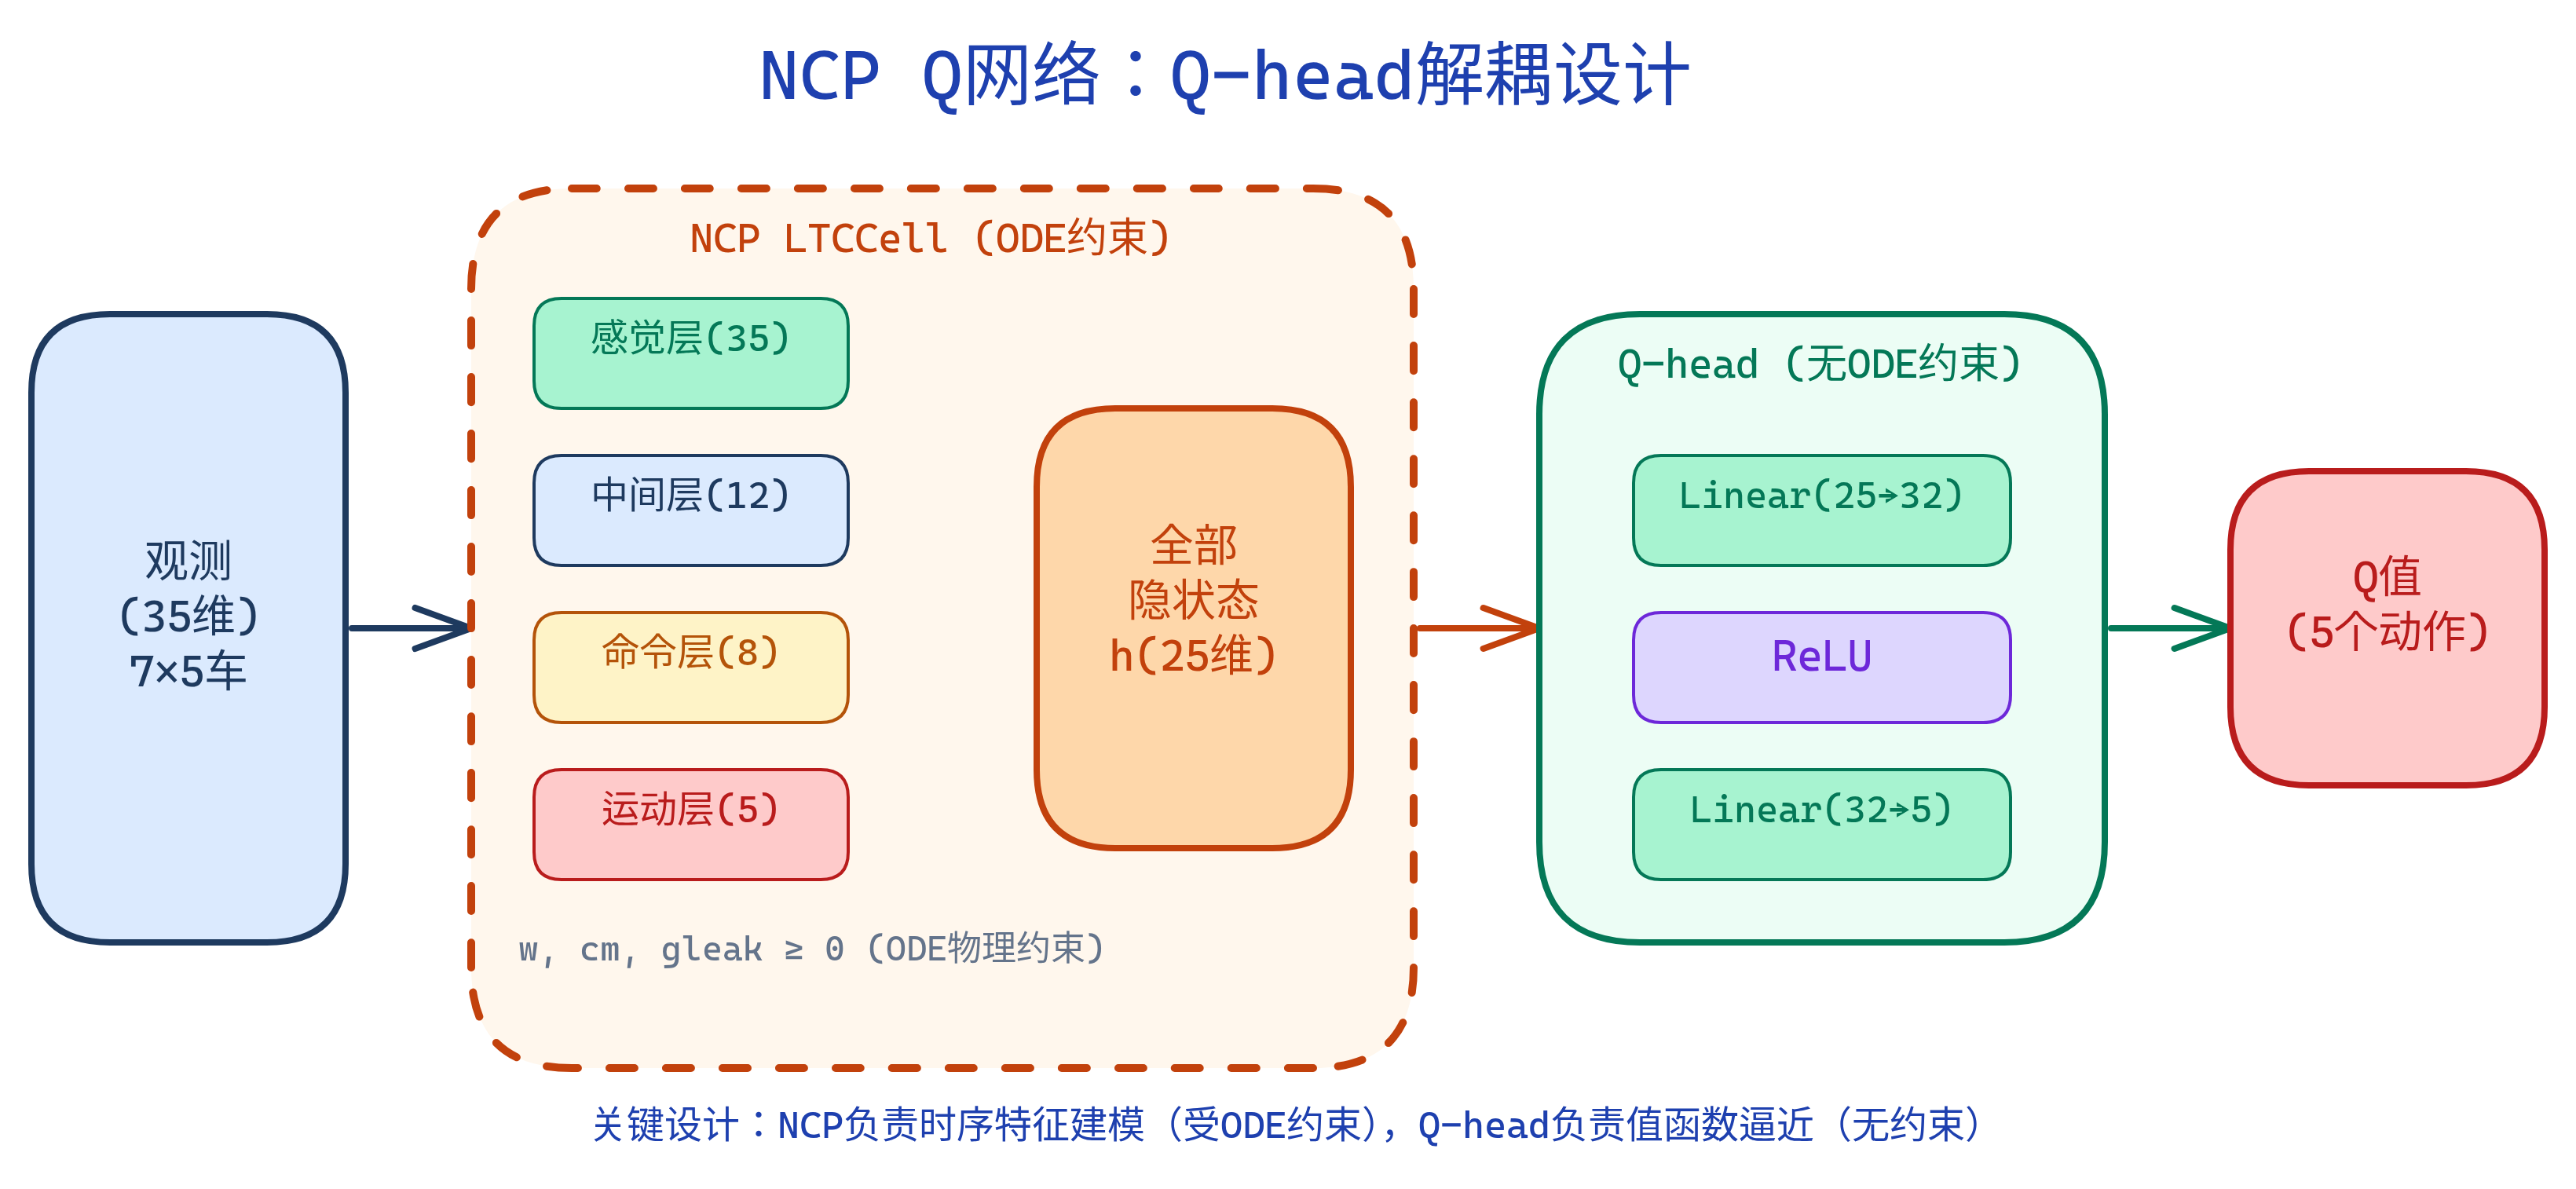
\includegraphics[width=0.9\linewidth]{img/fig_qhead.png}
    \caption{NCP Q网络的Q-head解耦设计}
    \label{fig:qhead}
\end{figure}

这种解耦设计的核心思想是：让NCP的ODE动力学专注于\textbf{时序特征建模}——通过液态时间常数捕捉驾驶场景的动态变化；让Q-head专注于\textbf{值函数逼近}——将NCP提取的动态特征映射为动作价值。两者分工明确，NCP的可解释性（稀疏结构、兴奋/抑制极性）得以完整保留，同时Q值估计不再受ODE约束的限制。

在训练过程中，NCP参数需要在每次梯度更新后执行权重裁剪（$w, c_m, g_{leak} \geq 0$），而Q-head参数不受此约束，两部分的梯度通过反向传播联合优化。
